\section{Datenvisualisierung}
Datenvisualisierung bedeutet Daten grafisch darzustellen. Dies ist ein erster Schritt in Machine Learning.\\
Visualisierung von Daten hilft um...
\begin{itemize}
\item ... ein intuitives Verständnis der Daten zu erhalten
\item ... Trends, clusters und lokale Muster zu sehen und identifizieren, welche man bei Raw-Daten sehr schwer sieht
\item ... Entdecken von Ausreissern und ungewöhnliche Gruppen
\item ...Trends zu identifizieren, cluster zu sehen
\item ..unsere Hypothesen/Vermutungen/Theorien zu validieren
\item ... Resultate von Umfragen, etc. zu visualisieren. (Dies sollte man bei wichtigen Nachrichten tun, da Leute meist nur die
\item Grafiken in einem Report ansehen, wenn sie diesen überfliegen.)
\end{itemize}
Datenvisualisierungen können auch überraschende Fakten aufdecken.
\subsection{Plots}
Mithilfe der Python Bibliotheken Mathplotlib und Seaborn (moderner, nutzerfreundlicher) können Daten visualisiert werden.
Um Daten zu importieren ist Pandas eine sehr hilfreiche Phyton-Bibliothek.\\
Ein Plot benötigt dringend nachfolgende Informationen:
\begin{itemize}
\item Label der X-Achse: Was für Daten werden in der X-Achse präsentiert?
\item Label der Y-Achse: Was für Daten werden in der Y-Achse präsentiert?
\item Titel: Was zeigt der Plot
\item Skala: Es muss entschieden werden zwischen Linear und Logarithmisch. Je nach dem andere Aussagekraft und besser geeignet. Beispiel Daten Moores Law: Transitoren pro Mikroprozessor. Hier ist logarithmisch besser geeignet, da es da es den Trend der Verdoppelung besser zeigt. Linear sieht so aus als wäre lange nichts passiert.
\item Dimension der Daten: 2D oder 3D ist das einzige was dargestellt werden kann und der Mensch auffassen kann. Mehr Dimensionen wie Wörtervektoren können nicht dargestellt werden oder müssen heruntergebrochen werden auf wenige Dimensionen
\end{itemize}

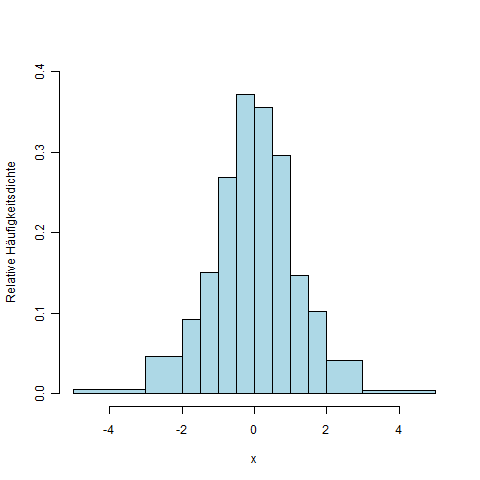
\includegraphics[width=\linewidth]{img/histogram.png}
Balken = Bins
\textcolor{myblue}{Box Plots und Violin Plots:}\\
Anzeigen von Daten anhand der Aufteilung in Quartile und Median. Zeigt sehr gut Aussreiser an und wo sich die meisten Daten befinden.
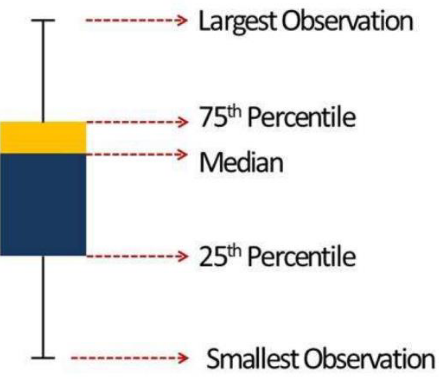
\includegraphics[width=0.9\linewidth]{img/boxplot.png}
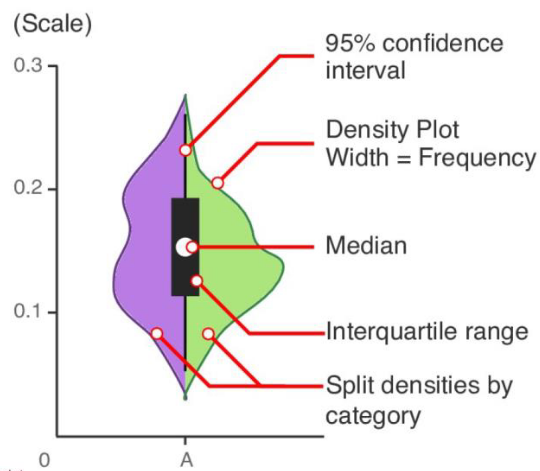
\includegraphics[width=0.9\linewidth]{img/violinplot.png}
\textcolor{myblue}{Streudiagramm (Scatter Plot)}\\
Zum Verständnis der Beziehung zwischen zwei kontinuierlichen Variablen kann ein Streudiagramm verwendet werden. Dabei kann eine Farbe verwendet werden um eine dritte Variable zu kodieren. Hilft dabei, eine Vorstellung vom Grad der Korrelation einer Variablen mit der anderen zu erhalten.
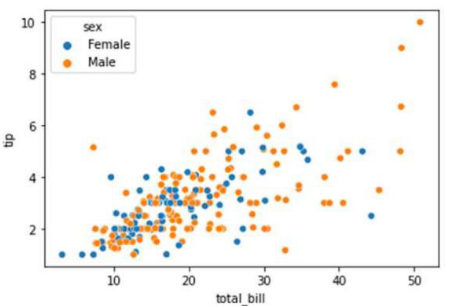
\includegraphics[width=\linewidth]{img/scatterplot.png}
\textcolor{myblue}{Auswahl Plot}\\
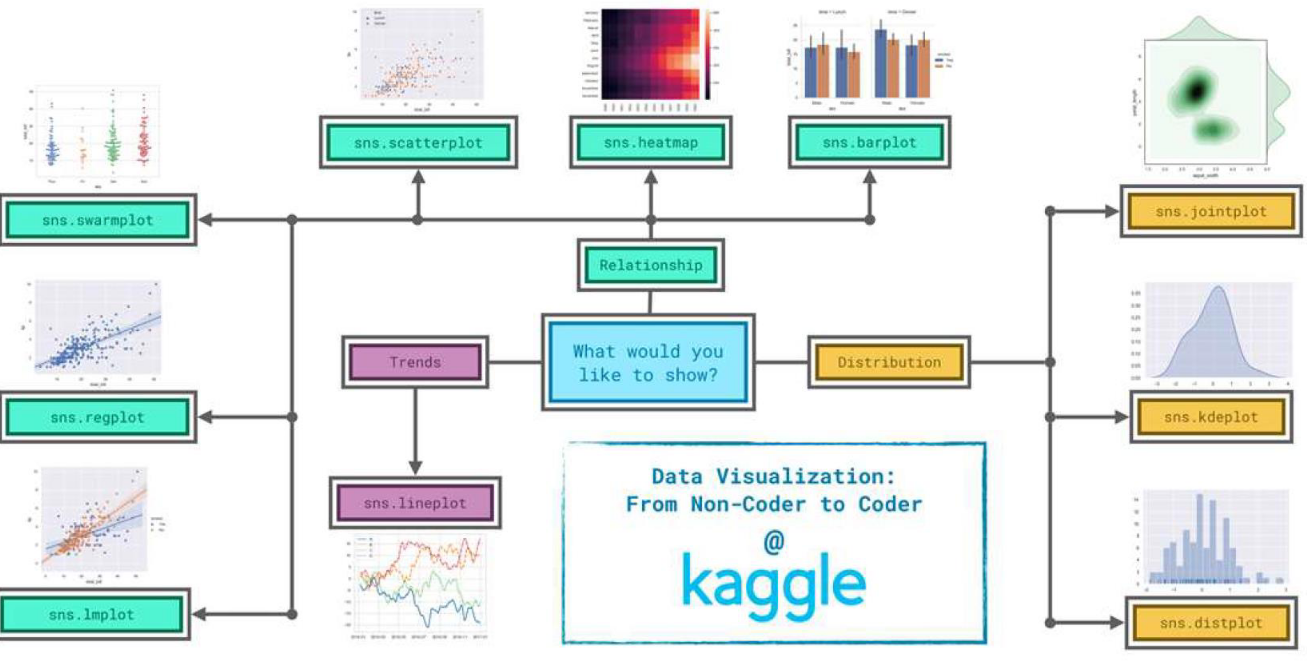
\includegraphics[width=\linewidth]{img/which_plot.png}